\section{Introduction}

\begin{figure}[t]
\centering
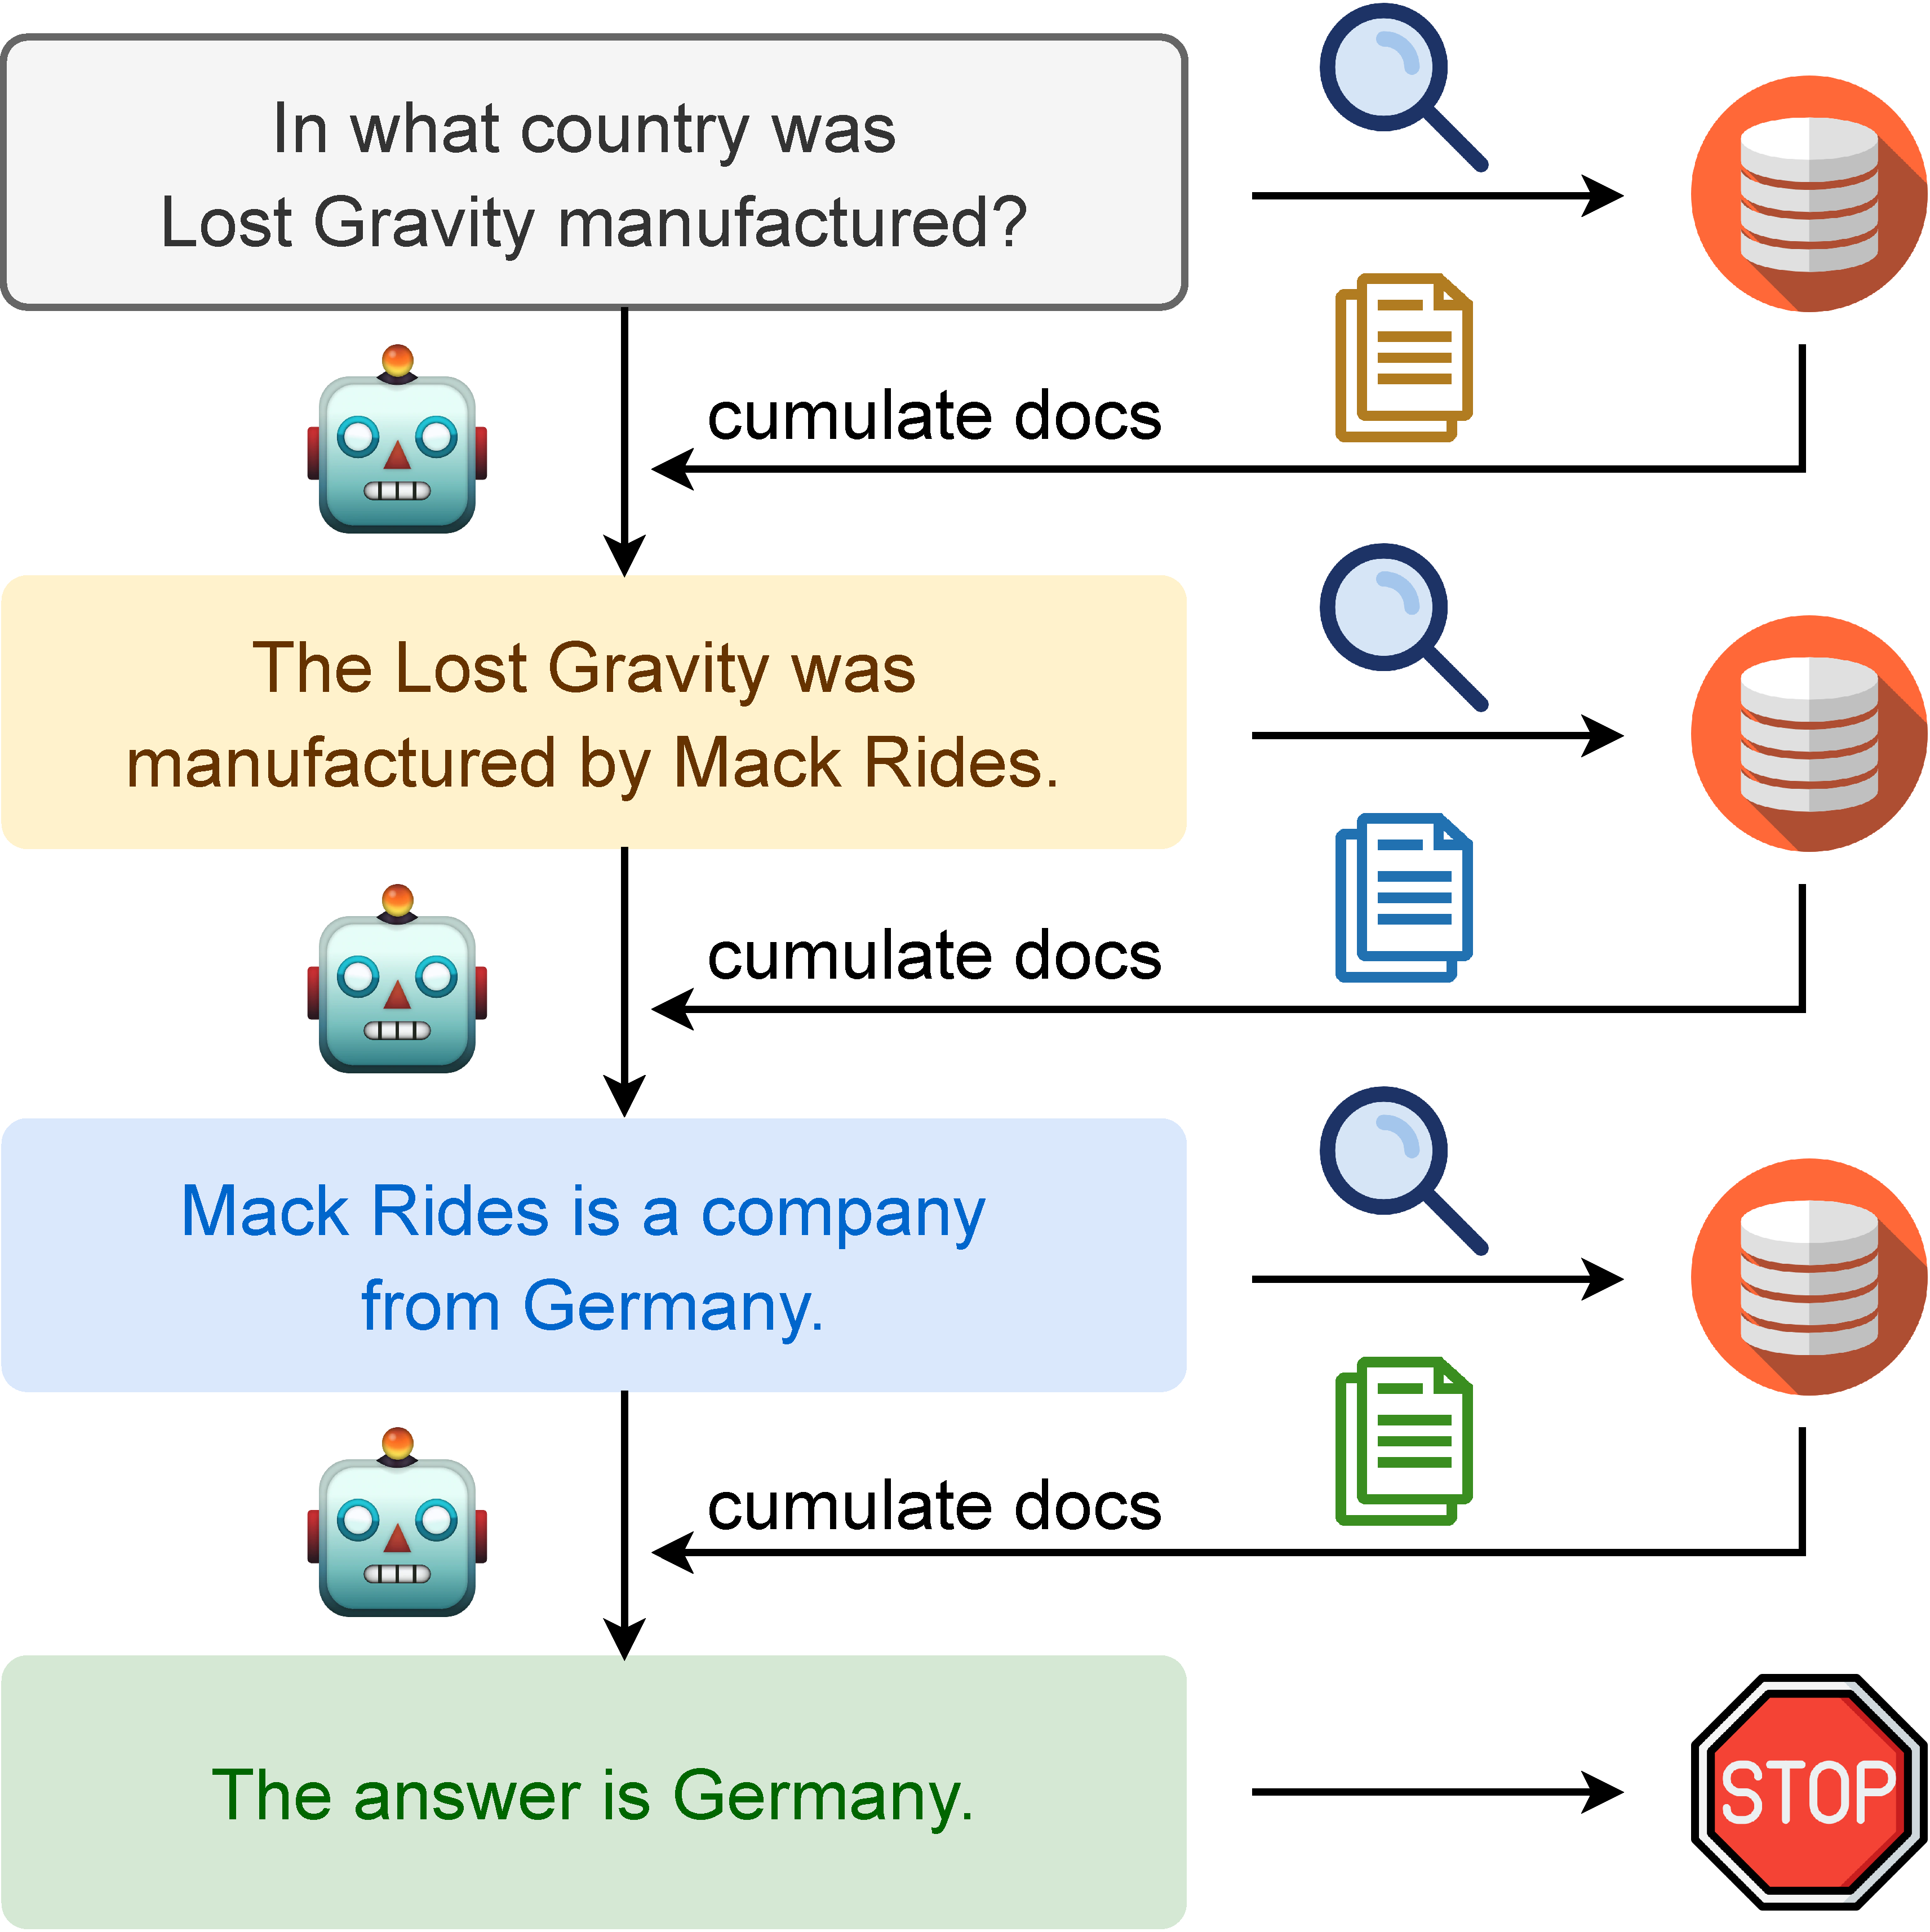
\includegraphics[width=0.45\textwidth]{images/intro-figure.pdf}
\caption{
\iconsys interleaves chain-of-thought (CoT) generation and knowledge retrieval steps in order to guide the retrieval by CoT and vice-versa. This interleaving allows retrieving more relevant information for later reasoning steps, compared to standard retrieval using solely the question as the query.}
\label{fig:intro-figure}
\end{figure}

Large language models are capable of answering complex questions by generating step-by-step natural language reasoning steps---so called chains of thoughts (CoT)---when prompted appropriately~\cite{cot}. This approach has been successful when all information needed to answer the question is either provided as context (e.g., algebra questions) or assumed to be present in the model's parameters (e.g., commonsense reasoning). However, for many open-domain questions, all required knowledge is not always available or up-to-date in models' parameters and it's beneficial to retrieve knowledge from external sources~\cite{internet-augmented-qa,realtime-qa}.


\emph{How can we augment chain-of-thought prompting for open-domain, knowledge-intensive tasks that require complex, multi-step reasoning?}

While a \textit{one-shot} retrieval from a knowledge source based solely on the question can successfully augment LMs with relevant knowledge for many factoid-based tasks~\cite{rag,realm,retro,atlas}, this strategy has clear limitations for more complex multi-step reasoning questions. For such questions, one often must retrieve partial knowledge, perform partial reasoning, retrieve additional information based on the outcome of the partial reasoning done so far, and iterate. 
As an example, consider the question illustrated in Fig.~\ref{fig:intro-figure}, \textit{``In what country was Lost Gravity manufactured?''}. The Wikipedia document retrieved using the question (in particular, the roller coaster Lost Gravity) as the query does not mention where Lost Gravity was manufactured. Instead, one must first infer that it was manufactured by a company called Mack Rides, and then perform further retrieval, guided by the inferred company name, to obtain evidence pointing to the manufacturing country.

Thus, the retrieval and reasoning steps must inform each other. Without retrieval, a model is likely to generate an incorrect reasoning step due to hallucination. Additionally, without generating the first reasoning step, the text supporting the second step can't be identified easily given the lack of lexical or even semantic overlap with the question. In other words, we need retrieved facts in order to generate factually correct reasoning steps and the reasoning steps to retrieve relevant facts.

Based on this intuition, we propose an \emph{interleaving approach} to this problem, where the idea is to use retrieval to guide the chain-of-thought (CoT) reasoning steps and use CoT reasoning to guide the retrieval. Fig.~\ref{fig:intro-figure} shows an overview of our retrieval method, which we call \iconsys.\footnote{\underline{I}nterleaved \underline{R}etrieval guided by \underline{C}hain-\underline{o}f-\underline{T}hought.} We begin by retrieving a base set of paragraphs using the question as a query. Subsequently, we alternate between the following two steps: (i) \textit{extend CoT}: use the question, the paragraphs collected thus far, and the CoT sentences generated thus far to generate the next CoT sentence; (ii) \textit{expand retrieved information}: use the last CoT sentence as a query to retrieve additional paragraphs to add to the collected set. We repeat these steps till the CoT reports an answer or we reach the maximum allowed number of reasoning steps. Upon termination, all collected paragraphs are returned as the retrieval outcome. Finally, we use these as the context for answering the question via direct QA prompting~\cite{originalgpt3} or CoT prompting~\cite{cot}.

We evaluate the efficacy of our system on 4 multi-step reasoning datasets under an open-domain setting: HotpotQA~\cite{hotpotqa}, 2WikiMultihopQA~\cite{xanh2020_2wikimultihop}, MuSiQue~\cite{musique}, and IIRC~\cite{iirc}. Our experiments using OpenAI GPT3 (\texttt{code-davinci-002}) \cite{originalgpt3,instructgpt3,codex} demonstrate that retrieval using \iconsys is substantially more effective than the baseline, one-step, question-based retrieval by 11-21 recall points under a fixed-budget optimal recall setup.\footnote{We explain later (in the Metric section and Footnote~\ref{footnote:retrieval-metric}) the appropriateness of this metric in our setting as opposed to more mainstream information recall metrics.} When \iconsys is used in conjunction with a prompting-based reader, it also leads to substantial improvement (up to 15 F1 points) in downstream few-shot QA performance and reduces factual errors in generated CoT by up to 50\%. Our approach also works on much smaller Flan-T5 models (11B, 3B, and 0.7B) showing similar trends. In particular, we find QA using Flan-T5-XL (3B) with \iconsys even outperforms the 58X larger GPT3 with a one-step question-based retrieval.
Furthermore, these improvements also hold up in an out-of-distribution (OOD) setting where the demonstrations from one dataset are used when testing on another dataset.
Lastly, we note that our QA scores exceed those reported by recent works on few-shot prompting for open-domain QA (ODQA)~\cite{decomp,selfask,react}, although a fair apples-to-apples comparison with them isn't possible (cf.~Appendix~\ref{sec:sota-differences}).

In summary, our main \textbf{contribution} is a novel retrieval method, \iconsys, that leverages LMs' chain-of-thought generation capabilities to guide retrieval and uses retrieval in turn to improve CoT reasoning. We demonstrate that \iconsys:
%
\begin{enumerate}[nosep]

    \item improves both retrieval and few-shot QA performance on several multi-step open-domain QA datasets, in both IID and OOD settings;

    \item reduces factual errors in generated CoTs; and

    \item improves performance with both large-scale (175B models) as well as smaller-scale models (Flan-T5-*, $\le$11B) without any training.

\end{enumerate}
